%%%%%%%%%%%%%%%%%%%%%%%%%%%%%%%%%%%%%%%%%%%%%%%%%%%%%%%%%%%%%
%% APPENDICES
%%%%%%%%%%%%%%%%%%%%%%%%%%%%%%%%%%%%%%%%%%%%%%%%%%%%%%%%%%%%%
\appendix

\chapter{Appendix}
\label{app:acronyms}
%% acronyms
\printindex
\printglossaries

\section{Data sets/Statistical Overview}
\label{app:data_sets}

\newpage
\section{MySQL Database}
\label{app:mysql_database}
\begin{figure}[ht]
	\centering
    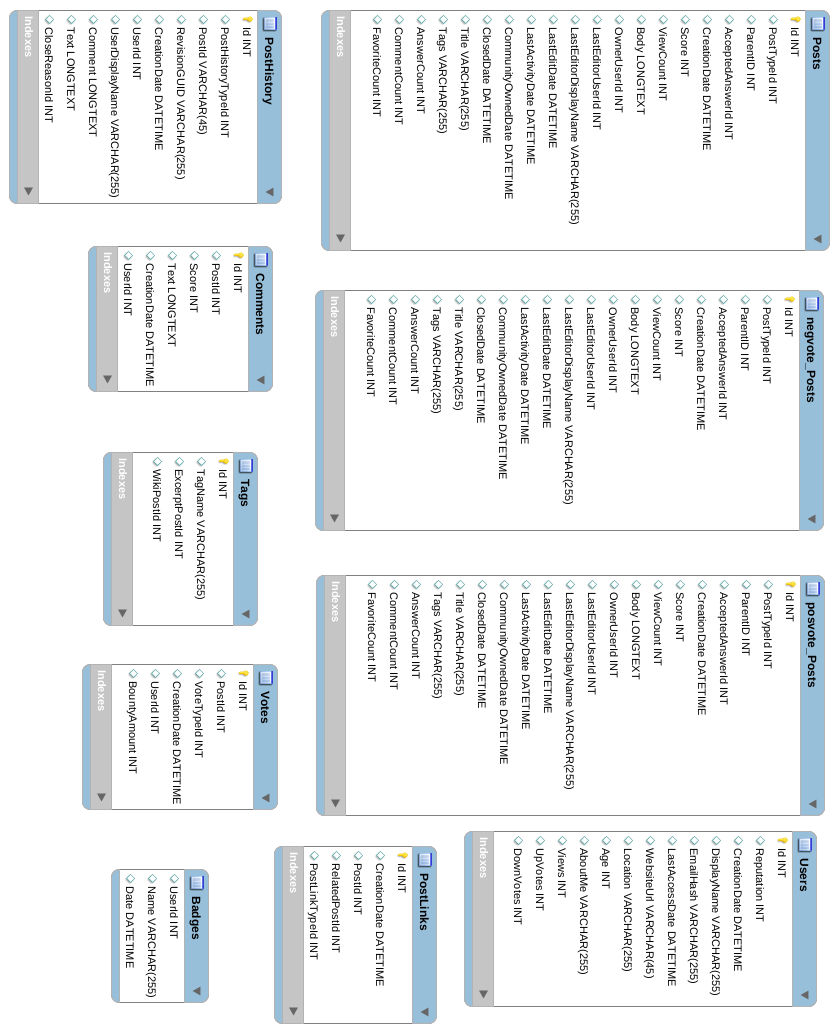
\includegraphics[width=0.8\textwidth]{so_database}
	\caption{MySQL Database used for dataset}
	\label{fig:mysql_database}
\end{figure}

% backup of various created tables


\begin{comment}
% potentially flip this, and this as a Score X feature (since all kernel values were the same)
% something like "Comparison ..., with Kernel = RBF, Gamma = gamma and C = c
% and the table having features as rows, and score X unprocessed as column
\begin{table}[tbp]
\centering
\begin{tabular}{| c | c | c | c | c | c | c | c |}
\hline
~ 					& Code sample	& Numerical		& Hexadecimal	& Homework		& Link 		& Tags	\\ \hline
Score 				& 0.783			& 0.796			& 0.793			& 0.794			& 0.795 	& 0.757	\\ \hline
C					& 1000			& 1000			& 1000			& 1000			& 1000 		& 1000	\\ \hline
Gamma ($\gamma$)	& 0.001			& 0.001			& 0.001			& 0.001			& 0.001 	& 0.001	\\ \hline
Kernel				& RBF			& RBF			& RBF			& RBF			& RBF 		& RBF	\\ \hline
\end{tabular}
\caption{Comparison of raw data set (unprocessed) and singular feature detectors}
%\label{tab:singular_feature_detector_so2}
\end{table}
\end{comment}

\begin{comment}
\begin{table}[tbp]
\centering
\begin{tabular}{| c | c | c | c | c |}
\hline
~				& Votes < 0			& Votes = 0			& Votes > 0		& All			\\ \hline
Amount			& 659,955			& 5,256,105			& 5,286,971		& 11,203,031	\\ \hline
Oldest			& 06.08.2008		& 06.08.2008		& 31.07.2008	& 31.07.2008 	\\ \hline
Newest			& 06.03.2016		& 06.03.2016		& 06.03.2016	& 06.03.2016	\\ \hline
Vote (lowest)	& -147				& 0					& 1				& -147	 		\\ \hline
Vote (highest)	& -1				& 0					& 13845			& 13845	 		\\ \hline
\end{tabular}
\caption{Overview of the Stack Overflow dataset.}
%\label{tab:dataset_overview_so2}
\end{table}
\end{comment}

\begin{comment}
Amount of features before anything was done to the text: 69766 - CountVectorizer(analyzer='word') - \%
Amount of features after adding stop word (English): 69462 - CountVectorizer(analyzer='word', stop\_words="english") - \%
Amount of features after removing code samples, hexadecimals and numeric values: 27624 - \%
Amount of features after setting minimum document frequency: 440 - CountVectorizer(analyzer='word', min\_df=0.01, stop_words='english') - \%


Originally tagged questions as good/bad, but then switched to +/-1 due to considering switching to LibSVM.
\end{comment}
